%% Los cap'itulos inician con \chapter{T'itulo}, estos aparecen numerados y
%% se incluyen en el 'indice general.
%%
%% Recuerda que aqu'i ya puedes escribir acentos como: 'a, 'e, 'i, etc.
%% La letra n con tilde es: 'n.

\chapter{Algoritmos de ordenamiento y mecanismos de manejo referencial}
\label{Algoritmos de ordenamiento y mecanismos del manejo referencial}
Una base de datos relacional esta fuertemente ligada al concepto Entidad Relaci\'on \cite{FBD}(E-R ``Entity Relationship"). Una entidad que representa gr\'aficamente a un concepto del mundo real o abstracta, que da lugar a una tabla en la base de datos. Una relaci\'on entre dos o m\'as entidades describe alguna interacci\'on entre las mismas, el tipo de relaci\'on  dar\'a lugar a un comportamiento entre las entidades involucradas \cite{introbasedatos}.

En un modelo Entidad Relaci\'on (E-R) para base de datos basados en ER Idioms\cite{idioms}, se tiene patrones de dise\~no m\'as definidos, las relaciones que llegan a tener entre entidades y la forma en que se hacen da lugar pr\'acticamente a los siguientes siete patrones de dise\~no para un modelo ER.
\begin{enumerate}
\item Una entidad que no hace referencia a otra pero si es referenciada es una entidad de tipo \textit{catalogo}. Act\'ua como un tipificador y generalmente almacenan peque\~nas cantidades de datos, los datos que se almacenan  se conocen a priori y la cantidades de datos son predecibles lo cual no significa que sean estables pueden llegar ha incrementarse, la entidad que hace referencia al \textit{catalogo} llega a ser una entidad de tipo \textit{catalogado}.
\item En algunos casos se tiene entidades que se encuentran sueltas por lo tanto no hacen referencia ni son referenciadas por ninguna otra, la cual es una entidad de tipo \textit{simple}.
\item En un modelo entidad relaci\'on donde una entidad hace referencia a m\'as de una y que su existencia depende de las mismas, a todo este conjunto se le denomina  \textit{composici\'on}.
\item
Cuando una entidad es dependiente de la existencia de otra al que detalla es de tipo \textit{detalle} de la alguna entidad maestra, donde el  detalle obedece a la maestra, a diferencia de un catalogador en un maestro no se puede determinar  los posibles datos a priori ni mucho menos estimar la cantidad aproximada de datos que pueda tener y que generalmente almacena cantidades grandes de datos.
\item
Hay veces que una entidad referencia a otra del mismo tipo llegando a ser una relaci\'on recursiva la cual llega a ser una entidad de tipo \textit{reflexivo simple}, cuando se implementa este tipo de relaci\'on es importante tener en cuenta que la relaci\'on no debe ser de obligatoriedad.
\item
En ocasiones es necesario relacionar entidades del mismo tipo y guardar un historial de ellas, la forma de representar este concepto es que una entidad representa la forma que se relacionan la entidad que hace una doble referencia, lo cual lleva a ser una entidad tipo  \textit{reflexivo compuesto}.
\item
Cuando se quiere hacer una especializaci\'on a una entidad en particular esta llega a ser la entidad hija de la entidad generalizada, este tipo de relaci\'on es conocida como \textit{is a} en idioms.
\end{enumerate}

\section{T\'ecnicas de ordenamiento}
En una base de datos las tablas tienen una secuencia de prioridades en el llenado de datos, una manera de obtener esta secuencia es buscar todas las tablas que no tengan ningun \texttt{foreign key}, posteriormente las tablas que tienen como \texttt{foreign key} que referencian a las anteriores y asi sucesivamente de manera secuencial, hasta acabar con el \'ultimo al que no referencia ninguna otra tabla, esto llega a ser confuso sobre todo si son muchas tablas al momento de hacer el llenado, para lo cual es necesario alguna t'ecnica para obtener el orden correcto del llenado en la base de datos.

La propuesta en este proyecto sobre la t\'ecnica para obtener el orden seg\'un la prioridad en que deben ser llenado las tablas con datos de prueba, es identificar primero todas aquellas que son una entidad tipo (\texttt{entity type}) catalogador, simple y  aquella que no tenga dependencia de ninguna otra, puede que en algunos casos est\'en los de tipo maestra  o las que son padre de una generalizaci\'on, los  sigu\'ientes a identificar son los catalogados, las que hacen referencia a las identificadas anteriormente pero que estas no deben depender de otras que a\'un no se llen\'o para evitar  tener problemas de inconsistencia.Un caso especial y para tener cuidado es la entidad tipo reflexivo simple, una entidad que hace referencia a uno de su mismo tipo con caracter\'isticas ya mencionadas anteriormente, este tipo de entidad va en la primera siempre que no haga referencia a una distinta de si misma.  
\section{Algoritmo de ordenamiento}
\label{Algoritmo de ordenamiento}
Para obtener la lista de tablas seg\'un el orden en que debe ser llenado una base de datos,  es necesario tener una lista capaz de almacenar elementos de diferentes contenido, esto debido a que el primer elemento puede ser un conjunto diferente al segundo para que es necesario aplicar el siguiente algoritmo:
\begin{enumerate}
\item Crear una lista de conjuntos.
\item Seleccionar las entidades de tipo catalogo, simple, maestra que no dependan de otra entidad y entidades que sean de tipo \textit{reflexivo simple}, que no hagan referencia a otra distinta de el, para luego almacenar este conjunto en la lista.
\item De la lista de conjuntos obtener el ultimo conjunto de entidades almacenada y por cada elemento buscar todas las entidades que le hagan referencia y que estas llegan a formar parte de otro conjunto de entidades, una vez recorrido todos los elementos agregar como un nuevo conjunto en la lista creada anteriormente.
\item Verificar que se ha recorrido todas las entidades, en caso de que se recorri\'o todo pasar al paso cinco, en caso contrario repetir el paso tres.
\item Si se llego hasta aqu\'i es porque se tiene la lista de conjuntos seg\'un a las dependencias, es decir  
un elemento de un conjunto referencia a otro elemento del conjunto anterior por lo tanto esta aun no es la lista. 

Ya que se da el caso de que el nombre de una entidad se repita en m\'as de una ocaci\'on dentro de un mismo conjunto o puede darse el caso que se repita el nombre en un conjunto anterior o posterior, por lo tanto es necesario aplicar el algoritmo de ordenaci\'on; primeros en ser llenados a la matriz de conjuntos. Antes de pasar al dicho algoritmo vease en un ejemplo en la siguiente secc\'ion.
\end{enumerate}
\section{Aplicaci\'on del algoritmo}

En la Figura \ref{fig:Modelo ER}, se tiene casos de tipos de entidades (\texttt{entity type}) seg\'un sea el caso se observa \texttt{PFK primary foreign key} llave foranea que a la vez es parte de la llave primaria, \texttt{PK primary key} llave primaria comunmente usadas en modelos ER Idioms.
\begin{figure}[H]
\centering
\subfigure{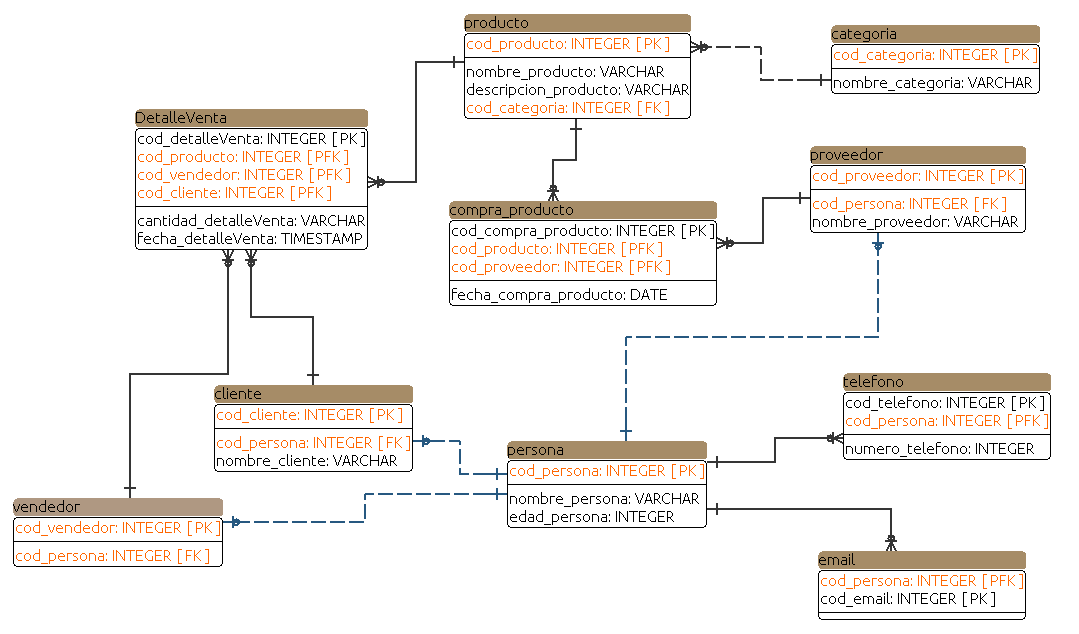
\includegraphics[scale=0.4]{images/modeloER}}
\caption{Ejemplo modelo ER} 
\label{fig:Modelo ER}
\end{figure}
Aplicando el paso dos del algoritmo se identifica una entidad catalogador \emph{categoria} y otra entidad que generaliza \emph{persona}, a partir ellas se busca los que le hacen referencia, \textit{categoria} y \textit{persona} llega a ser  la ra\'iz del \'arbol a generar, las entidades que hacen referencia serian \textit{(producto, cliente, vendedor, proveedor, telefono, email)} y un nivel mas abajo \textit{(detalleVenta y compra\_producto)}  aplicando el algoritmo se llega a la sigu\'iente Figura \ref{fig:ModeloOrdenado}.
\begin{figure}[H]
\centering
\subfigure{\includegraphics[scale=0.25]{images/arbol}}
\caption{Modelo Ordenado} \label{fig:ModeloOrdenado}
\end{figure}
\section{Algoritmo de ordenaci\'on \textit{primeros en ser llenado}}
\label{Algoritmo de ordenacion primeros en ser llenado}
Para obtener una lista de acuerdo al orden que se debe realizar el llenado, se inicia el recorrido de los conjuntos que trae la lista obtenida del algoritmo anterior, porque la lista se orden\'o seg\'un a que una entidad no dependiera de otra entidad, al recorrer se puede encontrar que una entidad se repita en distintos conjuntos, al  inicio de un conjunto, puede tambi\'en estar listada en medio o al final incluso se puede dar el caso que en un conjunto se repita m\'as de una ocac\'ion el nombre de una entidad. En la Figura \ref{fig:ModeloOrdenado} la entidad \textit{detalleVenta} se repite m\'as de una vez en la misma fila.

Entonces cual tomar como v\'alido?.
Para lo cual el  recorrido se comienza con el \'ultimo conjunto que tiene la lista, una vez encontrada las dem\'as que puedan encontrarse en posteriores no llegar\'a a ser v\'alida porque si bien hizo una referencia a un principio ser\'a valida el \'ultimo. Esto se justifica porque si se encuentra al \'ultimo es porque a\'un hace referencia a alg\'un elemento de la matriz anterior al que pertenece, por lo tanto se debi\'o esperar que se llegue hasta ese punto. para el caso de la Figura \ref{fig:ModeloOrdenado} listar el \'ultimo evitando que se repita.
Para obtener una lista ordenada seg\'un el orden en que deben ser llenados es necesario seguir la sigu\'iente secuencia de pasos:
\begin{enumerate}
\item Crear un matriz de tama\~no de la cantidad de entidades de la base de datos seleccionada.
\item Obtener el ultimo conjunto de entidades de la matriz.
\item Recorrer la matriz y verificar por cada elemento no exista en la matriz del paso uno, en caso de que no exista a\~nadir, de lo contrario no a\~nadir y pasar a la siguiente elemento.
\item Eliminar el ultimo conjunto de entidades de la matriz.
\item Si existen mas conjuntos de entidades en la matriz bidimensional volver a repetir el paso dos, caso contrario pasar al siguiente paso.
\item Invertir el orden de la matriz del paso uno.
\item Retornar la matriz creado en el paso uno que llegar\'ia a ser el orden que se requiere.
\end{enumerate}
\section{Aplicaci\'on del algoritmo de \textit{primeros en ser llenado}}
Con el algoritmo se llega a tener el siguiente orden en que debe ser llenado para el ejemplo dado en la figura  \ref{fig:Modelo ER}, el orden a seguir para este ejemplo es iniciar por el color verde terminando en el color rojo, el orden en cada fila no influye en el resultado permitiendo as\'i la flexibilidad de tomar cualquier elemento para el inicio de cada fila o el conjunto de elementos del mismo color.
\begin{figure}[H]
\centering
\subfigure{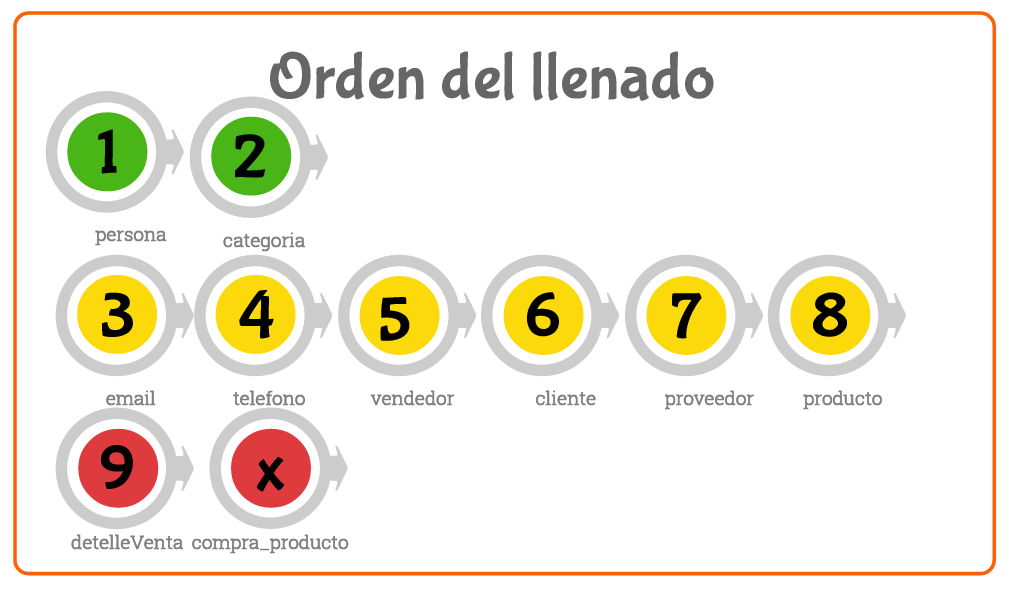
\includegraphics[scale=0.38]{images/ordenCorrecto}}
\caption{Orden de llenado}
\label{fig:Orden de llenado}
\end{figure}
\section{Mecanismo de \textit{manejo de referencial} de una base de datos}
Cuando un modelo entidad relaci\'on se lleva a un sistema gestor de base de datos, donde por cada entidad se crea una tabla y las  referencias son representadas mediante las llaves primarias y llaves for\'aneas, En caso de un modelo entidad relaci\'on basado en ER Idioms tiene ciertas caracter\'isticas que se explican en las siguientes subsecciones.
\subsection{Llaves primarias compuestas (\texttt{composite keys})}
Cuando se tiene m\'as de un \texttt{primary key}, entre ellas las que son propias de la tabla y otras pertenecientes a las que referencia que vienen como primarias, estan llegan a formar parte del \texttt{primary key} de la tabla, formando as'i \texttt{composite keys} para la misma. En conceptos de entidad relaci\'on en la figura  \ref{fig:llaves compuestas} se puede observar  las entidades que hacen referencia a otra.
Donde se puede ver que la entidad \textit{usuario\_rol} hace referencia a las entidades \textit{usuario} y \textit{rol}, las tres entidades llegar\'ian a formar una composici\'on  (\textit{usuario\_rol} compone de \textit{usuario} y \textit{rol}) donde la existencia de \textit{usuario\_rol} es dependiente de las que compone
\begin{figure}[H]
\centering
\subfigure{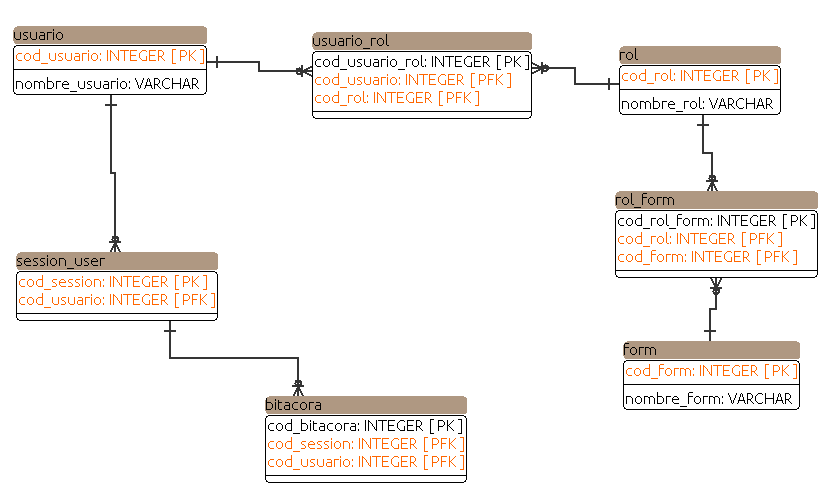
\includegraphics[scale=0.5]{images/llavesCompuestas}}
\caption{Llaves compuestas} \label{fig:llaves compuestas}
\end{figure}
Si este modelo se lleva a un gestor de base de datos un DBMS llega a tener como en el c\'odigo \ref{SQLtablaUsuarioRolComposite}.

\begin{lstlisting}[caption={SQL tabla usuario\_rol},label={SQLtablaUsuarioRolComposite},language=sql]
CREATE TABLE usuario_rol(
  cod_usuario_rol serial NOT NULL,
  cod_usuario INTEGER NOT NULL,
  cod_rol INTEGER NOT NULL,
  CONSTRAINT cod_usuario_rol PRIMARY KEY (cod_usuario_rol,cod_usuario,cod_rol),
  CONSTRAINT rol_usuario_rol_fk FOREIGN KEY (cod_rol)
      REFERENCES rol (cod_rol) MATCH SIMPLE
      ON UPDATE NOT ACTION ON DELETE NOT ACTION,
  CONSTRAINT usuario_usuario_rol_fk FOREIGN KEY (cod_usuario)
      REFERENCES usuario (cod_usuario) MATCH SIMPLE
      ON UPDATE NOT ACTION ON DELETE NOT ACTION
)
\end{lstlisting}
El \texttt{primary key} propia es independiente en cambio \textit{cod\_usuario} es perteneciente a la tabla \textit{usuario} pero viene como \texttt{primary key} lo mismo sucede con el campo \textit{cod\_rol}  que pertenece a la tabla \textit{rol}, como ambas \texttt{foreing key} vienen como \texttt{primary key} la tabla \textit{usuario\_rol} llegar'ia a tener un \texttt{primary key} compuesta de tres \textit{cod\_usuario\_rol, cod\_usuario, cod\_rol}. Cuando se quiere hacer una inserci\'on de un registro a la tabla \textit{usuario\_rol} sin antes haber realizado una inserci\'on a las tablas de \textit{usuario} y \textit{rol} cualquier DBMS no lo realiza la inserci\'on por razones de primero debe existir datos en las tablas.
\subsection{Mejor uso de Join}
El hacer uso de llaves compuestas(\texttt{composite keys}) hace que un identificador llegue m\'as all\'a de lo que normalmente se acostumbra vease en la figura  \ref{fig:llavesCompuestas}

Donde en la entidad bit\'acora se tiene tres \texttt{primary key} llega a ser una llave compuesta(\texttt{composite key}) y una de ellas es \textit{cod\_usuario} que si bien viene de \textit{session\_user} realmente su origen es en \textit{usuario}, por lo tanto se puede hacer un \texttt{join} entre \textit{bitacora} y \textit{usuario} evitando hacerlo con \textit{session\_user} obteniendo asi una consulta mas eficiente.
\begin{figure}[H]
\centering
\subfigure{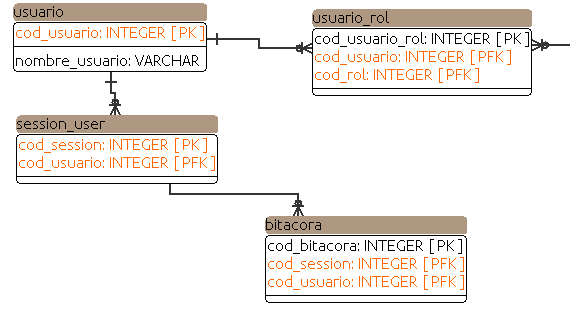
\includegraphics[scale=0.5]{images/join}}
\caption{Modelo E-R con llaves compuestas} \label{fig:llavesCompuestas}
\end{figure}
\section{Mecanismo de referenciaci\'on}
Cuando se genera datos de prueba para una base de datos es importante tener en cuenta el manejo de las llaves compuestas, no se puede generar al azar los \texttt{foreign key} porque se llegar'ia a tener problemas de inconsistencia.

Una t\'ecnica para evitar los problemas de inconsistencia es tener como fuente la tabla al que se referencia y los atributos de la tabla referenciada,  tomarlo como base para la generaci\'on de \emph{n} datos.
\subsection{Referencia simple}
Las referencias simples son cuando una tabla recibe solo un \texttt{primary key} o \texttt{foreign key} por parte de otra, en el c\'odigo \ref{lst:SQLUsuarioRolSimple} se puede observar el  \texttt{SQL} (por sus siglas en ingl\'es Structured Query Language) de la tabla \textit{usuario\_rol} de la figura \ref{fig:llaves compuestas}.  La tabla mencionada esta conformada de dos llaves que no son propias de la misma, \textit{cod\_usuario} forma parte de la tabla \textit{usuario} y \textit{cod\_rol} apunta a la tabla \textit{rol}, ambos son campos que apuntan a su respectiva tabla de manera \'unica, por lo tanto, se deja entender que se hace una referencia simple de llaves.

\begin{lstlisting}[caption={Referencia simple},label={lst:SQLUsuarioRolSimple},language=sql]
CREATE TABLE usuario_rol(
  cod_usuario_rol serial NOT NULL,
  cod_usuario INTEGER NOT NULL,
  cod_rol INTEGER NOT NULL,
  CONSTRAINT cod_usuario_rol PRIMARY KEY (cod_usuario_rol,cod_usuario,cod_rol),
  CONSTRAINT rol_usuario_rol_fk FOREIGN KEY (cod_rol)
      REFERENCES rol (cod_rol) MATCH SIMPLE
      ON UPDATE NOT ACTION ON DELETE NOT ACTION,
  CONSTRAINT usuario_usuario_rol_fk FOREIGN KEY (cod_usuario)
      REFERENCES usuario (cod_usuario) MATCH SIMPLE
      ON UPDATE NOT ACTION ON DELETE NOT ACTION
)
\end{lstlisting}
\subsection{Referencia compuesta}
La referencia compuesta ocurren cuando una tabla recibe m\'as de un \texttt{primary key} o \texttt{foreign key} por parte de otra. Es importante tomar los atributos que apuntan a otra como un conjunto de atributos para manejar como base para la generaci\'on de los datos requeridos.
\begin{lstlisting}[caption={Referencia compuesta},label={lst:SQLReferenciaCompuesta},language=sql]
CREATE TABLE bitacora(
  cod_bitacora serial NOT NULL,
  cod_session INTEGER NOT NULL,
  cod_usuario INTEGER NOT NULL,	  
  CONSTRAINT bitacora_pk PRIMARY KEY (cod_bitacora,cod_session,cod_usuario),
  CONSTRAINT session_user_bitacora_fk FOREIGN KEY (cod_session,cod_usuario)
      REFERENCES "session_user" (cod_session,cod_usuario) MATCH SIMPLE
      ON UPDATE NOT ACTION ON DELETE NOT ACTION
)
\end{lstlisting}
En el c\'odigo \ref{lst:SQLReferenciaCompuesta} el campo \textit{cod\_session} y \textit{cod\_usuario} de la tabla \textit{bitacora} hacen referencia a \textit{session\_user} a los campos \textit{cod\_session} y \textit{cod\_usuario}, son dos campos que referencia a la misma tabla, este caso \textit{session\_user} por lo tanto llega a ser una referencia compuesta.